\documentclass[1p]{elsarticle_modified}
%\bibliographystyle{elsarticle-num}

%\usepackage[colorlinks]{hyperref}
%\usepackage{abbrmath_seonhwa} %\Abb, \Ascr, \Acal ,\Abf, \Afrak
\usepackage{amsfonts}
\usepackage{amssymb}
\usepackage{amsmath}
\usepackage{amsthm}
\usepackage{scalefnt}
\usepackage{amsbsy}
\usepackage{kotex}
\usepackage{caption}
\usepackage{subfig}
\usepackage{color}
\usepackage{graphicx}
\usepackage{xcolor} %% white, black, red, green, blue, cyan, magenta, yellow
\usepackage{float}
\usepackage{setspace}
\usepackage{hyperref}

\usepackage{tikz}
\usetikzlibrary{arrows}

\usepackage{multirow}
\usepackage{array} % fixed length table
\usepackage{hhline}

%%%%%%%%%%%%%%%%%%%%%
\makeatletter
\renewcommand*\env@matrix[1][\arraystretch]{%
	\edef\arraystretch{#1}%
	\hskip -\arraycolsep
	\let\@ifnextchar\new@ifnextchar
	\array{*\c@MaxMatrixCols c}}
\makeatother %https://tex.stackexchange.com/questions/14071/how-can-i-increase-the-line-spacing-in-a-matrix
%%%%%%%%%%%%%%%

\usepackage[normalem]{ulem}

\newcommand{\msout}[1]{\ifmmode\text{\sout{\ensuremath{#1}}}\else\sout{#1}\fi}
%SOURCE: \msout is \stkout macro in https://tex.stackexchange.com/questions/20609/strikeout-in-math-mode

\newcommand{\cancel}[1]{
	\ifmmode
	{\color{red}\msout{#1}}
	\else
	{\color{red}\sout{#1}}
	\fi
}

\newcommand{\add}[1]{
	{\color{blue}\uwave{#1}}
}

\newcommand{\replace}[2]{
	\ifmmode
	{\color{red}\msout{#1}}{\color{blue}\uwave{#2}}
	\else
	{\color{red}\sout{#1}}{\color{blue}\uwave{#2}}
	\fi
}

\newcommand{\Sol}{\mathcal{S}} %segment
\newcommand{\D}{D} %diagram
\newcommand{\A}{\mathcal{A}} %arc


%%%%%%%%%%%%%%%%%%%%%%%%%%%%%5 test

\def\sl{\operatorname{\textup{SL}}(2,\Cbb)}
\def\psl{\operatorname{\textup{PSL}}(2,\Cbb)}
\def\quan{\mkern 1mu \triangleright \mkern 1mu}

\theoremstyle{definition}
\newtheorem{thm}{Theorem}[section]
\newtheorem{prop}[thm]{Proposition}
\newtheorem{lem}[thm]{Lemma}
\newtheorem{ques}[thm]{Question}
\newtheorem{cor}[thm]{Corollary}
\newtheorem{defn}[thm]{Definition}
\newtheorem{exam}[thm]{Example}
\newtheorem{rmk}[thm]{Remark}
\newtheorem{alg}[thm]{Algorithm}

\newcommand{\I}{\sqrt{-1}}
\begin{document}

%\begin{frontmatter}
%
%\title{Boundary parabolic representations of knots up to 8 crossings}
%
%%% Group authors per affiliation:
%\author{Yunhi Cho} 
%\address{Department of Mathematics, University of Seoul, Seoul, Korea}
%\ead{yhcho@uos.ac.kr}
%
%
%\author{Seonhwa Kim} %\fnref{s_kim}}
%\address{Center for Geometry and Physics, Institute for Basic Science, Pohang, 37673, Korea}
%\ead{ryeona17@ibs.re.kr}
%
%\author{Hyuk Kim}
%\address{Department of Mathematical Sciences, Seoul National University, Seoul 08826, Korea}
%\ead{hyukkim@snu.ac.kr}
%
%\author{Seokbeom Yoon}
%\address{Department of Mathematical Sciences, Seoul National University, Seoul, 08826,  Korea}
%\ead{sbyoon15@snu.ac.kr}
%
%\begin{abstract}
%We find all boundary parabolic representation of knots up to 8 crossings.
%
%\end{abstract}
%\begin{keyword}
%    \MSC[2010] 57M25 
%\end{keyword}
%
%\end{frontmatter}

%\linenumbers
%\tableofcontents
%
\newcommand\colored[1]{\textcolor{white}{\rule[-0.35ex]{0.8em}{1.4ex}}\kern-0.8em\color{red} #1}%
%\newcommand\colored[1]{\textcolor{white}{ #1}\kern-2.17ex	\textcolor{white}{ #1}\kern-1.81ex	\textcolor{white}{ #1}\kern-2.15ex\color{red}#1	}

{\Large $\underline{12a_{0037}~(K12a_{0037})}$}

\setlength{\tabcolsep}{10pt}
\renewcommand{\arraystretch}{1.6}
\vspace{1cm}\begin{tabular}{m{100pt}>{\centering\arraybackslash}m{274pt}}
\multirow{5}{120pt}{
	\centering
	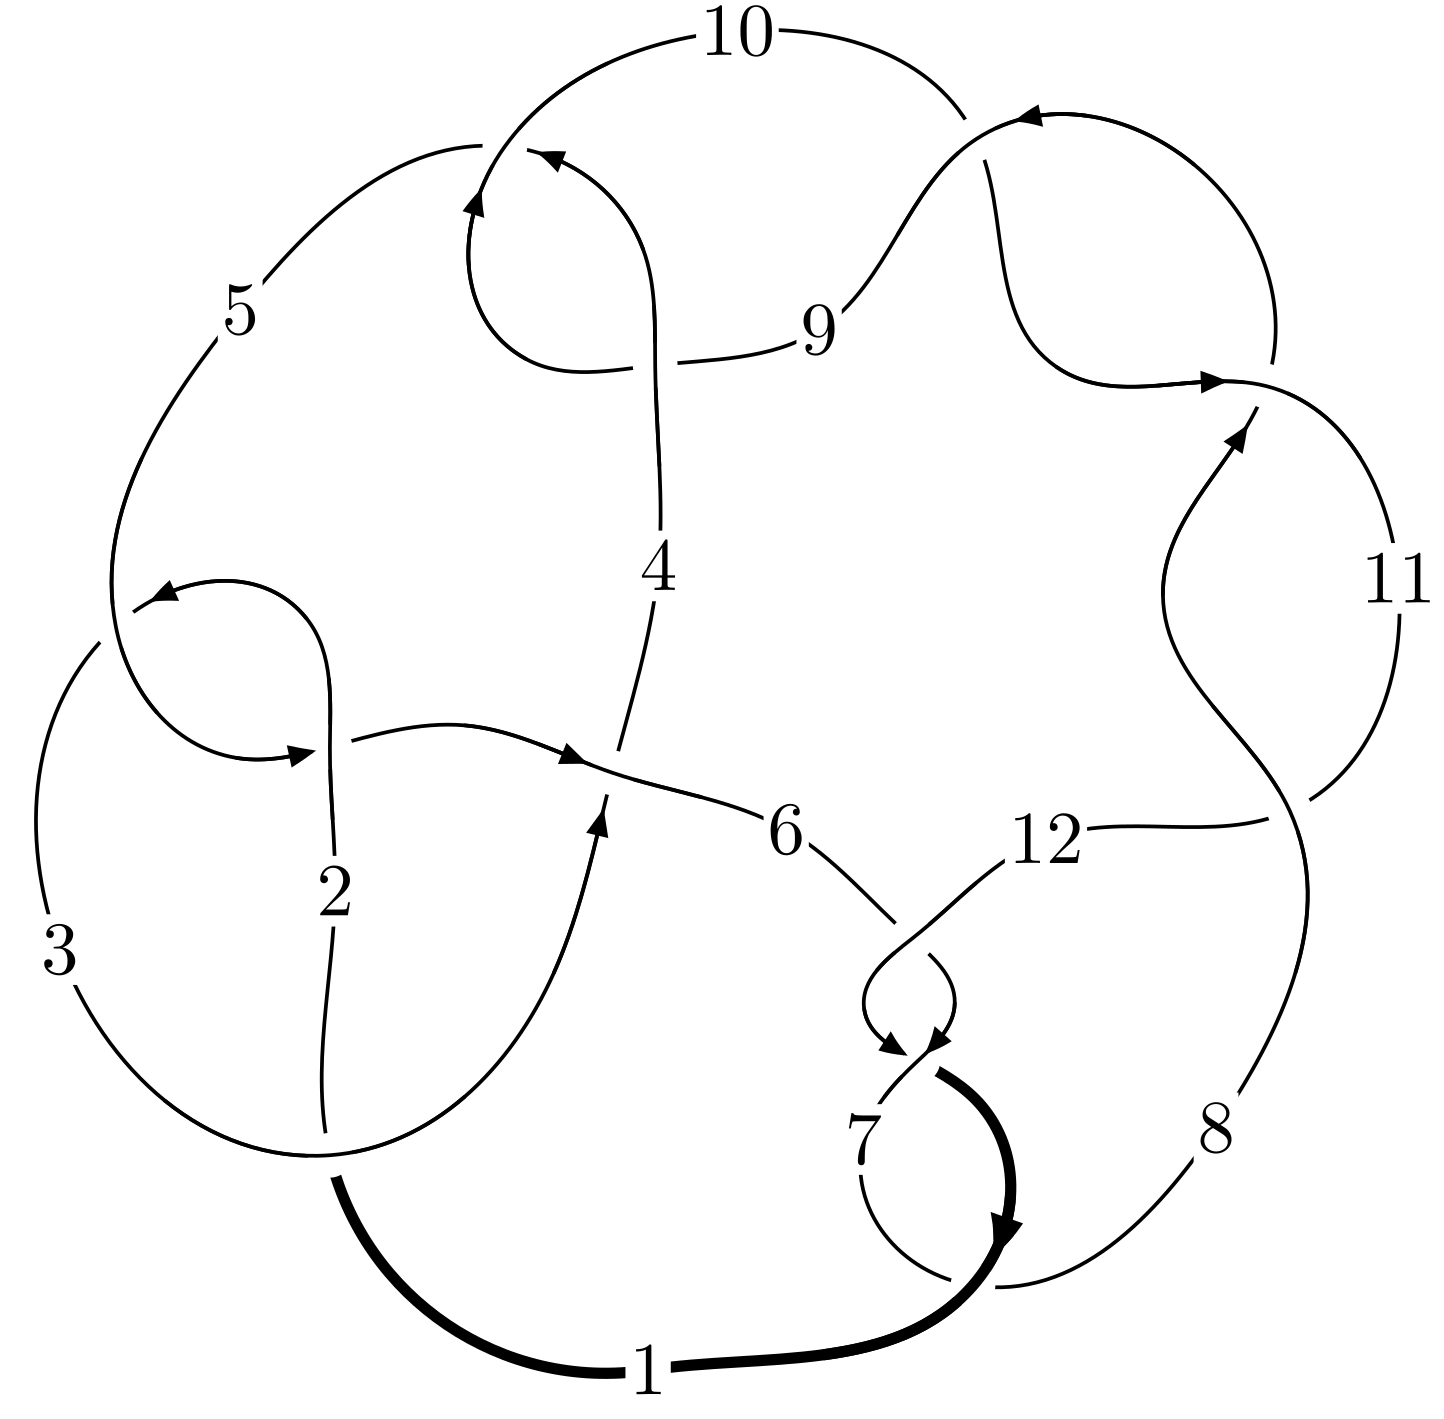
\includegraphics[width=112pt]{../../../GIT/diagram.site/Diagrams/png/838_12a_0037.png}\\
\ \ \ A knot diagram\footnotemark}&
\allowdisplaybreaks
\textbf{Linearized knot diagam} \\
\cline{2-2}
 &
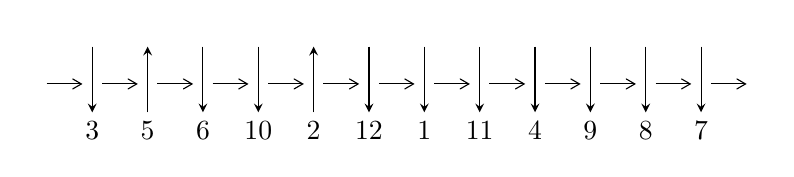
\begin{tikzpicture}[x=20pt, y=17pt]
	% nodes
	\node (C0) at (0, 0) {};
	\node (C1) at (1, 0) {};
	\node (C1U) at (1, +1) {};
	\node (C1D) at (1, -1) {3};

	\node (C2) at (2, 0) {};
	\node (C2U) at (2, +1) {};
	\node (C2D) at (2, -1) {5};

	\node (C3) at (3, 0) {};
	\node (C3U) at (3, +1) {};
	\node (C3D) at (3, -1) {6};

	\node (C4) at (4, 0) {};
	\node (C4U) at (4, +1) {};
	\node (C4D) at (4, -1) {10};

	\node (C5) at (5, 0) {};
	\node (C5U) at (5, +1) {};
	\node (C5D) at (5, -1) {2};

	\node (C6) at (6, 0) {};
	\node (C6U) at (6, +1) {};
	\node (C6D) at (6, -1) {12};

	\node (C7) at (7, 0) {};
	\node (C7U) at (7, +1) {};
	\node (C7D) at (7, -1) {1};

	\node (C8) at (8, 0) {};
	\node (C8U) at (8, +1) {};
	\node (C8D) at (8, -1) {11};

	\node (C9) at (9, 0) {};
	\node (C9U) at (9, +1) {};
	\node (C9D) at (9, -1) {4};

	\node (C10) at (10, 0) {};
	\node (C10U) at (10, +1) {};
	\node (C10D) at (10, -1) {9};

	\node (C11) at (11, 0) {};
	\node (C11U) at (11, +1) {};
	\node (C11D) at (11, -1) {8};

	\node (C12) at (12, 0) {};
	\node (C12U) at (12, +1) {};
	\node (C12D) at (12, -1) {7};
	\node (C13) at (13, 0) {};

	% arrows
	\draw[->,>={angle 60}]
	(C0) edge (C1) (C1) edge (C2) (C2) edge (C3) (C3) edge (C4) (C4) edge (C5) (C5) edge (C6) (C6) edge (C7) (C7) edge (C8) (C8) edge (C9) (C9) edge (C10) (C10) edge (C11) (C11) edge (C12) (C12) edge (C13) ;	\draw[->,>=stealth]
	(C1U) edge (C1D) (C2D) edge (C2U) (C3U) edge (C3D) (C4U) edge (C4D) (C5D) edge (C5U) (C6U) edge (C6D) (C7U) edge (C7D) (C8U) edge (C8D) (C9U) edge (C9D) (C10U) edge (C10D) (C11U) edge (C11D) (C12U) edge (C12D) ;
	\end{tikzpicture} \\
\hhline{~~} \\& 
\textbf{Solving Sequence} \\ \cline{2-2} 
 &
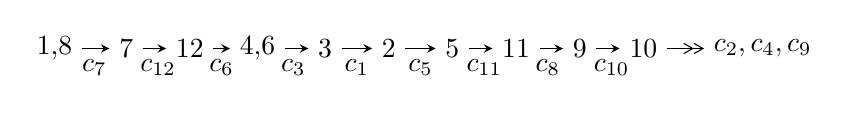
\begin{tikzpicture}[x=23pt, y=7pt]
	% node
	\node (A0) at (-1/8, 0) {1,8};
	\node (A1) at (1, 0) {7};
	\node (A2) at (2, 0) {12};
	\node (A3) at (49/16, 0) {4,6};
	\node (A4) at (33/8, 0) {3};
	\node (A5) at (41/8, 0) {2};
	\node (A6) at (49/8, 0) {5};
	\node (A7) at (57/8, 0) {11};
	\node (A8) at (65/8, 0) {9};
	\node (A9) at (73/8, 0) {10};
	\node (C1) at (1/2, -1) {$c_{7}$};
	\node (C2) at (3/2, -1) {$c_{12}$};
	\node (C3) at (5/2, -1) {$c_{6}$};
	\node (C4) at (29/8, -1) {$c_{3}$};
	\node (C5) at (37/8, -1) {$c_{1}$};
	\node (C6) at (45/8, -1) {$c_{5}$};
	\node (C7) at (53/8, -1) {$c_{11}$};
	\node (C8) at (61/8, -1) {$c_{8}$};
	\node (C9) at (69/8, -1) {$c_{10}$};
	\node (A10) at (11, 0) {$c_{2},c_{4},c_{9}$};

	% edge
	\draw[->,>=stealth]	
	(A0) edge (A1) (A1) edge (A2) (A2) edge (A3) (A3) edge (A4) (A4) edge (A5) (A5) edge (A6) (A6) edge (A7) (A7) edge (A8) (A8) edge (A9) ;
	\draw[->>,>={angle 60}]	
	(A9) edge (A10);
\end{tikzpicture} \\ 

\end{tabular} \\

\footnotetext{
The image of knot diagram is generated by the software ``\textbf{Draw programme}" developed by Andrew Bartholomew(\url{http://www.layer8.co.uk/maths/draw/index.htm\#Running-draw}), where we modified some parts for our purpose(\url{https://github.com/CATsTAILs/LinksPainter}).
}\phantom \\ \newline 
\centering \textbf{Ideals for irreducible components\footnotemark of $X_{\text{par}}$} 
 
\begin{align*}
I^u_{1}&=\langle 
3 u^{67}+5 u^{66}+\cdots+b-2,\;11 u^{67}+20 u^{66}+\cdots+2 a-9,\;u^{68}+3 u^{67}+\cdots- u-1\rangle \\
I^u_{2}&=\langle 
b,\;a^2+a+1,\;u-1\rangle \\
\\
\end{align*}
\raggedright * 2 irreducible components of $\dim_{\mathbb{C}}=0$, with total 70 representations.\\
\footnotetext{All coefficients of polynomials are rational numbers. But the coefficients are sometimes approximated in decimal forms when there is not enough margin.}
\newpage
\renewcommand{\arraystretch}{1}
\centering \section*{I. $I^u_{1}= \langle 3 u^{67}+5 u^{66}+\cdots+b-2,\;11 u^{67}+20 u^{66}+\cdots+2 a-9,\;u^{68}+3 u^{67}+\cdots- u-1 \rangle$}
\flushleft \textbf{(i) Arc colorings}\\
\begin{tabular}{m{7pt} m{180pt} m{7pt} m{180pt} }
\flushright $a_{1}=$&$\begin{pmatrix}0\\u\end{pmatrix}$ \\
\flushright $a_{8}=$&$\begin{pmatrix}1\\0\end{pmatrix}$ \\
\flushright $a_{7}=$&$\begin{pmatrix}1\\- u^2\end{pmatrix}$ \\
\flushright $a_{12}=$&$\begin{pmatrix}u\\- u^3+u\end{pmatrix}$ \\
\flushright $a_{4}=$&$\begin{pmatrix}-\frac{11}{2} u^{67}-10 u^{66}+\cdots-2 u+\frac{9}{2}\\-3 u^{67}-5 u^{66}+\cdots-11 u^2+2\end{pmatrix}$ \\
\flushright $a_{6}=$&$\begin{pmatrix}- u^2+1\\u^4-2 u^2\end{pmatrix}$ \\
\flushright $a_{3}=$&$\begin{pmatrix}-\frac{7}{2} u^{67}-6 u^{66}+\cdots-3 u+\frac{5}{2}\\\frac{1}{2} u^{67}+u^{66}+\cdots- u-\frac{1}{2}\end{pmatrix}$ \\
\flushright $a_{2}=$&$\begin{pmatrix}-\frac{1}{2} u^{67}- u^{66}+\cdots+8 u-\frac{1}{2}\\\frac{1}{2} u^{67}+u^{66}+\cdots+2 u-\frac{1}{2}\end{pmatrix}$ \\
\flushright $a_{5}=$&$\begin{pmatrix}-\frac{5}{2} u^{67}-4 u^{66}+\cdots- u+\frac{5}{2}\\6 u^{67}+11 u^{66}+\cdots- u-5\end{pmatrix}$ \\
\flushright $a_{11}=$&$\begin{pmatrix}- u^3+2 u\\- u^3+u\end{pmatrix}$ \\
\flushright $a_{9}=$&$\begin{pmatrix}u^6-3 u^4+2 u^2+1\\u^6-2 u^4+u^2\end{pmatrix}$ \\
\flushright $a_{10}=$&$\begin{pmatrix}- u^9+4 u^7-5 u^5+3 u\\- u^9+3 u^7-3 u^5+u\end{pmatrix}$\\&\end{tabular}
\flushleft \textbf{(ii) Obstruction class $= -1$}\\~\\
\flushleft \textbf{(iii) Cusp Shapes $= 14 u^{67}+19 u^{66}+\cdots-9 u-17$}\\~\\
\newpage\renewcommand{\arraystretch}{1}
\flushleft \textbf{(iv) u-Polynomials at the component}\newline \\
\begin{tabular}{m{50pt}|m{274pt}}
Crossings & \hspace{64pt}u-Polynomials at each crossing \\
\hline $$\begin{aligned}c_{1}\end{aligned}$$&$\begin{aligned}
&u^{68}+30 u^{67}+\cdots-2 u+1
\end{aligned}$\\
\hline $$\begin{aligned}c_{2},c_{5}\end{aligned}$$&$\begin{aligned}
&u^{68}+2 u^{67}+\cdots+6 u+1
\end{aligned}$\\
\hline $$\begin{aligned}c_{3}\end{aligned}$$&$\begin{aligned}
&u^{68}-2 u^{67}+\cdots-36 u+9
\end{aligned}$\\
\hline $$\begin{aligned}c_{4},c_{9}\end{aligned}$$&$\begin{aligned}
&u^{68}+u^{67}+\cdots-8 u-4
\end{aligned}$\\
\hline $$\begin{aligned}c_{6},c_{7},c_{12}\end{aligned}$$&$\begin{aligned}
&u^{68}-3 u^{67}+\cdots+u-1
\end{aligned}$\\
\hline $$\begin{aligned}c_{8},c_{10},c_{11}\end{aligned}$$&$\begin{aligned}
&u^{68}+15 u^{67}+\cdots+152 u+16
\end{aligned}$\\
\hline
\end{tabular}\\~\\
\newpage\renewcommand{\arraystretch}{1}
\flushleft \textbf{(v) Riley Polynomials at the component}\newline \\
\begin{tabular}{m{50pt}|m{274pt}}
Crossings & \hspace{64pt}Riley Polynomials at each crossing \\
\hline $$\begin{aligned}c_{1}\end{aligned}$$&$\begin{aligned}
&y^{68}+18 y^{67}+\cdots-62 y+1
\end{aligned}$\\
\hline $$\begin{aligned}c_{2},c_{5}\end{aligned}$$&$\begin{aligned}
&y^{68}+30 y^{67}+\cdots-2 y+1
\end{aligned}$\\
\hline $$\begin{aligned}c_{3}\end{aligned}$$&$\begin{aligned}
&y^{68}+6 y^{67}+\cdots+4014 y+81
\end{aligned}$\\
\hline $$\begin{aligned}c_{4},c_{9}\end{aligned}$$&$\begin{aligned}
&y^{68}-15 y^{67}+\cdots-152 y+16
\end{aligned}$\\
\hline $$\begin{aligned}c_{6},c_{7},c_{12}\end{aligned}$$&$\begin{aligned}
&y^{68}-53 y^{67}+\cdots-13 y+1
\end{aligned}$\\
\hline $$\begin{aligned}c_{8},c_{10},c_{11}\end{aligned}$$&$\begin{aligned}
&y^{68}+73 y^{67}+\cdots-2592 y+256
\end{aligned}$\\
\hline
\end{tabular}\\~\\
\newpage\flushleft \textbf{(vi) Complex Volumes and Cusp Shapes}
$$\begin{array}{c|c|c}  
\text{Solutions to }I^u_{1}& \I (\text{vol} + \sqrt{-1}CS) & \text{Cusp shape}\\
 \hline 
\begin{aligned}
u &= \phantom{-}0.895522 + 0.351354 I \\
a &= \phantom{-}0.535572 - 0.466640 I \\
b &= \phantom{-}0.419390 - 0.166116 I\end{aligned}
 & -2.40466 + 3.24426 I & -12.79487 + 0. I\phantom{ +0.000000I} \\ \hline\begin{aligned}
u &= \phantom{-}0.895522 - 0.351354 I \\
a &= \phantom{-}0.535572 + 0.466640 I \\
b &= \phantom{-}0.419390 + 0.166116 I\end{aligned}
 & -2.40466 - 3.24426 I & -12.79487 + 0. I\phantom{ +0.000000I} \\ \hline\begin{aligned}
u &= \phantom{-}1.030920 + 0.245142 I \\
a &= -0.144942 + 0.300433 I \\
b &= -0.536018 + 0.056317 I\end{aligned}
 & -0.929775 - 0.694625 I & \phantom{-0.000000 } 0 \\ \hline\begin{aligned}
u &= \phantom{-}1.030920 - 0.245142 I \\
a &= -0.144942 - 0.300433 I \\
b &= -0.536018 - 0.056317 I\end{aligned}
 & -0.929775 + 0.694625 I & \phantom{-0.000000 } 0 \\ \hline\begin{aligned}
u &= \phantom{-}0.057827 + 0.908622 I \\
a &= -1.03946 - 2.62331 I \\
b &= -0.97261 - 2.56092 I\end{aligned}
 & \phantom{-}7.88380 - 10.29650 I & -4.69943 + 7.27910 I \\ \hline\begin{aligned}
u &= \phantom{-}0.057827 - 0.908622 I \\
a &= -1.03946 + 2.62331 I \\
b &= -0.97261 + 2.56092 I\end{aligned}
 & \phantom{-}7.88380 + 10.29650 I & -4.69943 - 7.27910 I \\ \hline\begin{aligned}
u &= \phantom{-}0.042720 + 0.903115 I \\
a &= \phantom{-}0.65870 + 2.72612 I \\
b &= \phantom{-}0.70317 + 2.64498 I\end{aligned}
 & \phantom{-}9.72190 - 4.90561 I & -2.02313 + 2.74922 I \\ \hline\begin{aligned}
u &= \phantom{-}0.042720 - 0.903115 I \\
a &= \phantom{-}0.65870 - 2.72612 I \\
b &= \phantom{-}0.70317 - 2.64498 I\end{aligned}
 & \phantom{-}9.72190 + 4.90561 I & -2.02313 - 2.74922 I \\ \hline\begin{aligned}
u &= \phantom{-}0.003428 + 0.888270 I \\
a &= -0.34321 + 2.84573 I \\
b &= -0.00404 + 2.75361 I\end{aligned}
 & \phantom{-}9.88596 - 1.57474 I & -1.66767 + 2.29520 I \\ \hline\begin{aligned}
u &= \phantom{-}0.003428 - 0.888270 I \\
a &= -0.34321 - 2.84573 I \\
b &= -0.00404 - 2.75361 I\end{aligned}
 & \phantom{-}9.88596 + 1.57474 I & -1.66767 - 2.29520 I\\
 \hline 
 \end{array}$$\newpage$$\begin{array}{c|c|c}  
\text{Solutions to }I^u_{1}& \I (\text{vol} + \sqrt{-1}CS) & \text{Cusp shape}\\
 \hline 
\begin{aligned}
u &= -0.013729 + 0.881119 I \\
a &= \phantom{-}0.78129 - 2.82252 I \\
b &= \phantom{-}0.31193 - 2.74554 I\end{aligned}
 & \phantom{-}8.18285 + 3.81988 I & -4.00036 - 2.43227 I \\ \hline\begin{aligned}
u &= -0.013729 - 0.881119 I \\
a &= \phantom{-}0.78129 + 2.82252 I \\
b &= \phantom{-}0.31193 + 2.74554 I\end{aligned}
 & \phantom{-}8.18285 - 3.81988 I & -4.00036 + 2.43227 I \\ \hline\begin{aligned}
u &= \phantom{-}0.040273 + 0.862504 I \\
a &= -0.13886 - 1.98365 I \\
b &= -0.31232 - 2.13385 I\end{aligned}
 & \phantom{-}4.10183 - 3.09420 I & -7.72899 + 2.66205 I \\ \hline\begin{aligned}
u &= \phantom{-}0.040273 - 0.862504 I \\
a &= -0.13886 + 1.98365 I \\
b &= -0.31232 + 2.13385 I\end{aligned}
 & \phantom{-}4.10183 + 3.09420 I & -7.72899 - 2.66205 I \\ \hline\begin{aligned}
u &= -1.186300 + 0.127926 I \\
a &= -0.90918 - 1.24102 I \\
b &= \phantom{-}0.436322 - 0.125183 I\end{aligned}
 & -2.19445 - 0.93220 I & \phantom{-0.000000 } 0 \\ \hline\begin{aligned}
u &= -1.186300 - 0.127926 I \\
a &= -0.90918 + 1.24102 I \\
b &= \phantom{-}0.436322 + 0.125183 I\end{aligned}
 & -2.19445 + 0.93220 I & \phantom{-0.000000 } 0 \\ \hline\begin{aligned}
u &= \phantom{-}1.187500 + 0.181105 I \\
a &= -0.228112 + 0.140426 I \\
b &= -1.199570 + 0.450826 I\end{aligned}
 & -1.34633 - 1.22738 I & \phantom{-0.000000 } 0 \\ \hline\begin{aligned}
u &= \phantom{-}1.187500 - 0.181105 I \\
a &= -0.228112 - 0.140426 I \\
b &= -1.199570 - 0.450826 I\end{aligned}
 & -1.34633 + 1.22738 I & \phantom{-0.000000 } 0 \\ \hline\begin{aligned}
u &= -1.213540 + 0.182772 I \\
a &= \phantom{-}0.391833 + 1.256010 I \\
b &= -0.311997 + 0.100144 I\end{aligned}
 & -1.54755 + 4.00408 I & \phantom{-0.000000 } 0 \\ \hline\begin{aligned}
u &= -1.213540 - 0.182772 I \\
a &= \phantom{-}0.391833 - 1.256010 I \\
b &= -0.311997 - 0.100144 I\end{aligned}
 & -1.54755 - 4.00408 I & \phantom{-0.000000 } 0\\
 \hline 
 \end{array}$$\newpage$$\begin{array}{c|c|c}  
\text{Solutions to }I^u_{1}& \I (\text{vol} + \sqrt{-1}CS) & \text{Cusp shape}\\
 \hline 
\begin{aligned}
u &= \phantom{-}1.247790 + 0.069716 I \\
a &= \phantom{-}0.262311 - 0.505966 I \\
b &= \phantom{-}0.81938 - 1.63973 I\end{aligned}
 & -4.41264 + 1.01414 I & \phantom{-0.000000 } 0 \\ \hline\begin{aligned}
u &= \phantom{-}1.247790 - 0.069716 I \\
a &= \phantom{-}0.262311 + 0.505966 I \\
b &= \phantom{-}0.81938 + 1.63973 I\end{aligned}
 & -4.41264 - 1.01414 I & \phantom{-0.000000 } 0 \\ \hline\begin{aligned}
u &= \phantom{-}0.626055 + 0.376261 I \\
a &= \phantom{-}0.779550 + 0.334297 I \\
b &= \phantom{-}0.620215 - 0.009222 I\end{aligned}
 & -3.00525 - 2.85440 I & -15.4568 + 5.4193 I \\ \hline\begin{aligned}
u &= \phantom{-}0.626055 - 0.376261 I \\
a &= \phantom{-}0.779550 - 0.334297 I \\
b &= \phantom{-}0.620215 + 0.009222 I\end{aligned}
 & -3.00525 + 2.85440 I & -15.4568 - 5.4193 I \\ \hline\begin{aligned}
u &= \phantom{-}1.260630 + 0.174920 I \\
a &= \phantom{-}0.502698 - 0.114267 I \\
b &= \phantom{-}1.88463 - 0.84447 I\end{aligned}
 & -3.25504 - 5.41820 I & \phantom{-0.000000 } 0 \\ \hline\begin{aligned}
u &= \phantom{-}1.260630 - 0.174920 I \\
a &= \phantom{-}0.502698 + 0.114267 I \\
b &= \phantom{-}1.88463 + 0.84447 I\end{aligned}
 & -3.25504 + 5.41820 I & \phantom{-0.000000 } 0 \\ \hline\begin{aligned}
u &= \phantom{-}0.260329 + 0.674892 I \\
a &= \phantom{-}0.059835 - 1.200510 I \\
b &= \phantom{-}0.036602 - 0.171621 I\end{aligned}
 & -0.54570 - 7.12975 I & -8.28357 + 9.67470 I \\ \hline\begin{aligned}
u &= \phantom{-}0.260329 - 0.674892 I \\
a &= \phantom{-}0.059835 + 1.200510 I \\
b &= \phantom{-}0.036602 + 0.171621 I\end{aligned}
 & -0.54570 + 7.12975 I & -8.28357 - 9.67470 I \\ \hline\begin{aligned}
u &= \phantom{-}1.239520 + 0.401715 I \\
a &= \phantom{-}1.098620 - 0.433220 I \\
b &= -0.64232 - 1.99545 I\end{aligned}
 & \phantom{-}0.39705 - 1.43860 I & \phantom{-0.000000 } 0 \\ \hline\begin{aligned}
u &= \phantom{-}1.239520 - 0.401715 I \\
a &= \phantom{-}1.098620 + 0.433220 I \\
b &= -0.64232 + 1.99545 I\end{aligned}
 & \phantom{-}0.39705 + 1.43860 I & \phantom{-0.000000 } 0\\
 \hline 
 \end{array}$$\newpage$$\begin{array}{c|c|c}  
\text{Solutions to }I^u_{1}& \I (\text{vol} + \sqrt{-1}CS) & \text{Cusp shape}\\
 \hline 
\begin{aligned}
u &= \phantom{-}1.232810 + 0.456922 I \\
a &= \phantom{-}1.83683 - 0.03858 I \\
b &= \phantom{-}0.38520 - 2.25306 I\end{aligned}
 & \phantom{-}4.26036 + 5.42868 I & \phantom{-0.000000 } 0 \\ \hline\begin{aligned}
u &= \phantom{-}1.232810 - 0.456922 I \\
a &= \phantom{-}1.83683 + 0.03858 I \\
b &= \phantom{-}0.38520 + 2.25306 I\end{aligned}
 & \phantom{-}4.26036 - 5.42868 I & \phantom{-0.000000 } 0 \\ \hline\begin{aligned}
u &= -1.32040\phantom{ +0.000000I} \\
a &= -0.354230\phantom{ +0.000000I} \\
b &= \phantom{-}0.972963\phantom{ +0.000000I}\end{aligned}
 & -6.07475\phantom{ +0.000000I} & \phantom{-0.000000 } 0 \\ \hline\begin{aligned}
u &= \phantom{-}1.245710 + 0.445929 I \\
a &= -1.76468 + 0.31816 I \\
b &= -0.09620 + 2.45581 I\end{aligned}
 & \phantom{-}6.00508 + 0.09093 I & \phantom{-0.000000 } 0 \\ \hline\begin{aligned}
u &= \phantom{-}1.245710 - 0.445929 I \\
a &= -1.76468 - 0.31816 I \\
b &= -0.09620 - 2.45581 I\end{aligned}
 & \phantom{-}6.00508 - 0.09093 I & \phantom{-0.000000 } 0 \\ \hline\begin{aligned}
u &= -1.313060 + 0.227651 I \\
a &= \phantom{-}0.198042 + 0.731027 I \\
b &= \phantom{-}0.288228 + 0.423614 I\end{aligned}
 & -3.29836 + 5.64762 I & \phantom{-0.000000 } 0 \\ \hline\begin{aligned}
u &= -1.313060 - 0.227651 I \\
a &= \phantom{-}0.198042 - 0.731027 I \\
b &= \phantom{-}0.288228 - 0.423614 I\end{aligned}
 & -3.29836 - 5.64762 I & \phantom{-0.000000 } 0 \\ \hline\begin{aligned}
u &= -1.266290 + 0.417661 I \\
a &= -1.99000 - 0.31891 I \\
b &= \phantom{-}0.23911 - 2.26817 I\end{aligned}
 & \phantom{-}4.29886 + 0.82820 I & \phantom{-0.000000 } 0 \\ \hline\begin{aligned}
u &= -1.266290 - 0.417661 I \\
a &= -1.99000 + 0.31891 I \\
b &= \phantom{-}0.23911 + 2.26817 I\end{aligned}
 & \phantom{-}4.29886 - 0.82820 I & \phantom{-0.000000 } 0 \\ \hline\begin{aligned}
u &= \phantom{-}1.276200 + 0.421764 I \\
a &= -1.50037 + 0.93745 I \\
b &= \phantom{-}0.67185 + 2.85731 I\end{aligned}
 & \phantom{-}5.93444 - 3.11164 I & \phantom{-0.000000 } 0\\
 \hline 
 \end{array}$$\newpage$$\begin{array}{c|c|c}  
\text{Solutions to }I^u_{1}& \I (\text{vol} + \sqrt{-1}CS) & \text{Cusp shape}\\
 \hline 
\begin{aligned}
u &= \phantom{-}1.276200 - 0.421764 I \\
a &= -1.50037 - 0.93745 I \\
b &= \phantom{-}0.67185 - 2.85731 I\end{aligned}
 & \phantom{-}5.93444 + 3.11164 I & \phantom{-0.000000 } 0 \\ \hline\begin{aligned}
u &= \phantom{-}0.194231 + 0.624177 I \\
a &= \phantom{-}0.200700 + 0.974073 I \\
b &= \phantom{-}0.166804 - 0.050748 I\end{aligned}
 & \phantom{-}1.39398 - 2.63459 I & -3.83138 + 5.30336 I \\ \hline\begin{aligned}
u &= \phantom{-}0.194231 - 0.624177 I \\
a &= \phantom{-}0.200700 - 0.974073 I \\
b &= \phantom{-}0.166804 + 0.050748 I\end{aligned}
 & \phantom{-}1.39398 + 2.63459 I & -3.83138 - 5.30336 I \\ \hline\begin{aligned}
u &= -1.281690 + 0.420235 I \\
a &= \phantom{-}1.86247 + 0.63495 I \\
b &= -0.54582 + 2.40594 I\end{aligned}
 & \phantom{-}5.89281 + 6.25632 I & \phantom{-0.000000 } 0 \\ \hline\begin{aligned}
u &= -1.281690 - 0.420235 I \\
a &= \phantom{-}1.86247 - 0.63495 I \\
b &= -0.54582 - 2.40594 I\end{aligned}
 & \phantom{-}5.89281 - 6.25632 I & \phantom{-0.000000 } 0 \\ \hline\begin{aligned}
u &= -1.339060 + 0.171690 I \\
a &= -0.296922 - 0.787136 I \\
b &= \phantom{-}0.164287 - 0.826587 I\end{aligned}
 & -7.45261 + 2.99913 I & \phantom{-0.000000 } 0 \\ \hline\begin{aligned}
u &= -1.339060 - 0.171690 I \\
a &= -0.296922 + 0.787136 I \\
b &= \phantom{-}0.164287 + 0.826587 I\end{aligned}
 & -7.45261 - 2.99913 I & \phantom{-0.000000 } 0 \\ \hline\begin{aligned}
u &= \phantom{-}1.288500 + 0.412732 I \\
a &= \phantom{-}1.35888 - 1.17047 I \\
b &= -1.01417 - 2.98905 I\end{aligned}
 & \phantom{-}4.13145 - 8.45277 I & \phantom{-0.000000 } 0 \\ \hline\begin{aligned}
u &= \phantom{-}1.288500 - 0.412732 I \\
a &= \phantom{-}1.35888 + 1.17047 I \\
b &= -1.01417 + 2.98905 I\end{aligned}
 & \phantom{-}4.13145 + 8.45277 I & \phantom{-0.000000 } 0 \\ \hline\begin{aligned}
u &= -1.305290 + 0.396523 I \\
a &= -1.154370 - 0.714946 I \\
b &= \phantom{-}1.13010 - 1.94509 I\end{aligned}
 & -0.09743 + 7.61245 I & \phantom{-0.000000 } 0\\
 \hline 
 \end{array}$$\newpage$$\begin{array}{c|c|c}  
\text{Solutions to }I^u_{1}& \I (\text{vol} + \sqrt{-1}CS) & \text{Cusp shape}\\
 \hline 
\begin{aligned}
u &= -1.305290 - 0.396523 I \\
a &= -1.154370 + 0.714946 I \\
b &= \phantom{-}1.13010 + 1.94509 I\end{aligned}
 & -0.09743 - 7.61245 I & \phantom{-0.000000 } 0 \\ \hline\begin{aligned}
u &= -1.364380 + 0.036473 I \\
a &= \phantom{-}0.061668 + 0.259510 I \\
b &= -1.252540 + 0.333167 I\end{aligned}
 & -9.10989 + 3.71218 I & \phantom{-0.000000 } 0 \\ \hline\begin{aligned}
u &= -1.364380 - 0.036473 I \\
a &= \phantom{-}0.061668 - 0.259510 I \\
b &= -1.252540 - 0.333167 I\end{aligned}
 & -9.10989 - 3.71218 I & \phantom{-0.000000 } 0 \\ \hline\begin{aligned}
u &= -1.347280 + 0.239850 I \\
a &= -0.322191 - 0.625658 I \\
b &= -0.620089 - 0.700964 I\end{aligned}
 & -5.60593 + 10.34200 I & \phantom{-0.000000 } 0 \\ \hline\begin{aligned}
u &= -1.347280 - 0.239850 I \\
a &= -0.322191 + 0.625658 I \\
b &= -0.620089 + 0.700964 I\end{aligned}
 & -5.60593 - 10.34200 I & \phantom{-0.000000 } 0 \\ \hline\begin{aligned}
u &= \phantom{-}0.352806 + 0.523351 I \\
a &= -0.429659 - 1.178270 I \\
b &= -0.416900 - 0.230397 I\end{aligned}
 & -2.23370 - 0.62660 I & -12.61670 + 3.83528 I \\ \hline\begin{aligned}
u &= \phantom{-}0.352806 - 0.523351 I \\
a &= -0.429659 + 1.178270 I \\
b &= -0.416900 + 0.230397 I\end{aligned}
 & -2.23370 + 0.62660 I & -12.61670 - 3.83528 I \\ \hline\begin{aligned}
u &= -1.313460 + 0.421883 I \\
a &= \phantom{-}1.43757 + 1.23124 I \\
b &= -1.29435 + 2.56292 I\end{aligned}
 & \phantom{-}5.48960 + 9.64527 I & \phantom{-0.000000 } 0 \\ \hline\begin{aligned}
u &= -1.313460 - 0.421883 I \\
a &= \phantom{-}1.43757 - 1.23124 I \\
b &= -1.29435 - 2.56292 I\end{aligned}
 & \phantom{-}5.48960 - 9.64527 I & \phantom{-0.000000 } 0 \\ \hline\begin{aligned}
u &= -1.324500 + 0.421925 I \\
a &= -1.24973 - 1.42112 I \\
b &= \phantom{-}1.58602 - 2.58289 I\end{aligned}
 & \phantom{-}3.5636 + 15.0559 I & \phantom{-0.000000 } 0\\
 \hline 
 \end{array}$$\newpage$$\begin{array}{c|c|c}  
\text{Solutions to }I^u_{1}& \I (\text{vol} + \sqrt{-1}CS) & \text{Cusp shape}\\
 \hline 
\begin{aligned}
u &= -1.324500 - 0.421925 I \\
a &= -1.24973 + 1.42112 I \\
b &= \phantom{-}1.58602 + 2.58289 I\end{aligned}
 & \phantom{-}3.5636 - 15.0559 I & \phantom{-0.000000 } 0 \\ \hline\begin{aligned}
u &= \phantom{-}0.013858 + 0.538053 I \\
a &= \phantom{-}0.93729 + 1.22313 I \\
b &= \phantom{-}0.676344 - 0.109112 I\end{aligned}
 & \phantom{-}2.08272 - 1.40752 I & -0.96646 + 3.79117 I \\ \hline\begin{aligned}
u &= \phantom{-}0.013858 - 0.538053 I \\
a &= \phantom{-}0.93729 - 1.22313 I \\
b &= \phantom{-}0.676344 + 0.109112 I\end{aligned}
 & \phantom{-}2.08272 + 1.40752 I & -0.96646 - 3.79117 I \\ \hline\begin{aligned}
u &= -0.099088 + 0.477326 I \\
a &= -1.27945 - 1.92708 I \\
b &= -0.871503 - 0.181323 I\end{aligned}
 & \phantom{-}0.87080 + 3.06361 I & -3.02049 - 3.15038 I \\ \hline\begin{aligned}
u &= -0.099088 - 0.477326 I \\
a &= -1.27945 + 1.92708 I \\
b &= -0.871503 + 0.181323 I\end{aligned}
 & \phantom{-}0.87080 - 3.06361 I & -3.02049 + 3.15038 I \\ \hline\begin{aligned}
u &= \phantom{-}0.440851\phantom{ +0.000000I} \\
a &= \phantom{-}0.0522081\phantom{ +0.000000I} \\
b &= -0.459473\phantom{ +0.000000I}\end{aligned}
 & -0.831706\phantom{ +0.000000I} & -11.9310\phantom{ +0.000000I} \\ \hline\begin{aligned}
u &= -0.189182 + 0.115386 I \\
a &= -0.02171 - 3.59531 I \\
b &= -0.205879 - 0.531302 I\end{aligned}
 & -0.30583 - 1.79467 I & -2.23312 + 3.53008 I \\ \hline\begin{aligned}
u &= -0.189182 - 0.115386 I \\
a &= -0.02171 + 3.59531 I \\
b &= -0.205879 + 0.531302 I\end{aligned}
 & -0.30583 + 1.79467 I & -2.23312 - 3.53008 I\\
 \hline 
 \end{array}$$\newpage\newpage\renewcommand{\arraystretch}{1}
\centering \section*{II. $I^u_{2}= \langle b,\;a^2+a+1,\;u-1 \rangle$}
\flushleft \textbf{(i) Arc colorings}\\
\begin{tabular}{m{7pt} m{180pt} m{7pt} m{180pt} }
\flushright $a_{1}=$&$\begin{pmatrix}0\\1\end{pmatrix}$ \\
\flushright $a_{8}=$&$\begin{pmatrix}1\\0\end{pmatrix}$ \\
\flushright $a_{7}=$&$\begin{pmatrix}1\\-1\end{pmatrix}$ \\
\flushright $a_{12}=$&$\begin{pmatrix}1\\0\end{pmatrix}$ \\
\flushright $a_{4}=$&$\begin{pmatrix}a\\0\end{pmatrix}$ \\
\flushright $a_{6}=$&$\begin{pmatrix}0\\-1\end{pmatrix}$ \\
\flushright $a_{3}=$&$\begin{pmatrix}a\\- a\end{pmatrix}$ \\
\flushright $a_{2}=$&$\begin{pmatrix}a+1\\- a\end{pmatrix}$ \\
\flushright $a_{5}=$&$\begin{pmatrix}a\\0\end{pmatrix}$ \\
\flushright $a_{11}=$&$\begin{pmatrix}1\\0\end{pmatrix}$ \\
\flushright $a_{9}=$&$\begin{pmatrix}1\\0\end{pmatrix}$ \\
\flushright $a_{10}=$&$\begin{pmatrix}1\\0\end{pmatrix}$\\&\end{tabular}
\flushleft \textbf{(ii) Obstruction class $= 1$}\\~\\
\flushleft \textbf{(iii) Cusp Shapes $= -4 a-11$}\\~\\
\newpage\renewcommand{\arraystretch}{1}
\flushleft \textbf{(iv) u-Polynomials at the component}\newline \\
\begin{tabular}{m{50pt}|m{274pt}}
Crossings & \hspace{64pt}u-Polynomials at each crossing \\
\hline $$\begin{aligned}c_{1},c_{3},c_{5}\end{aligned}$$&$\begin{aligned}
&u^2- u+1
\end{aligned}$\\
\hline $$\begin{aligned}c_{2}\end{aligned}$$&$\begin{aligned}
&u^2+u+1
\end{aligned}$\\
\hline $$\begin{aligned}c_{4},c_{8},c_{9}\\c_{10},c_{11}\end{aligned}$$&$\begin{aligned}
&u^2
\end{aligned}$\\
\hline $$\begin{aligned}c_{6},c_{7}\end{aligned}$$&$\begin{aligned}
&(u-1)^2
\end{aligned}$\\
\hline $$\begin{aligned}c_{12}\end{aligned}$$&$\begin{aligned}
&(u+1)^2
\end{aligned}$\\
\hline
\end{tabular}\\~\\
\newpage\renewcommand{\arraystretch}{1}
\flushleft \textbf{(v) Riley Polynomials at the component}\newline \\
\begin{tabular}{m{50pt}|m{274pt}}
Crossings & \hspace{64pt}Riley Polynomials at each crossing \\
\hline $$\begin{aligned}c_{1},c_{2},c_{3}\\c_{5}\end{aligned}$$&$\begin{aligned}
&y^2+y+1
\end{aligned}$\\
\hline $$\begin{aligned}c_{4},c_{8},c_{9}\\c_{10},c_{11}\end{aligned}$$&$\begin{aligned}
&y^2
\end{aligned}$\\
\hline $$\begin{aligned}c_{6},c_{7},c_{12}\end{aligned}$$&$\begin{aligned}
&(y-1)^2
\end{aligned}$\\
\hline
\end{tabular}\\~\\
\newpage\flushleft \textbf{(vi) Complex Volumes and Cusp Shapes}
$$\begin{array}{c|c|c}  
\text{Solutions to }I^u_{2}& \I (\text{vol} + \sqrt{-1}CS) & \text{Cusp shape}\\
 \hline 
\begin{aligned}
u &= \phantom{-}1.00000\phantom{ +0.000000I} \\
a &= -0.500000 + 0.866025 I \\
b &= \phantom{-0.000000 } 0\end{aligned}
 & -1.64493 + 2.02988 I & -9.00000 - 3.46410 I \\ \hline\begin{aligned}
u &= \phantom{-}1.00000\phantom{ +0.000000I} \\
a &= -0.500000 - 0.866025 I \\
b &= \phantom{-0.000000 } 0\end{aligned}
 & -1.64493 - 2.02988 I & -9.00000 + 3.46410 I\\
 \hline 
 \end{array}$$\newpage
\newpage\renewcommand{\arraystretch}{1}
\centering \section*{ III. u-Polynomials}
\begin{tabular}{m{50pt}|m{274pt}}
Crossings & \hspace{64pt}u-Polynomials at each crossing \\
\hline $$\begin{aligned}c_{1}\end{aligned}$$&$\begin{aligned}
&(u^2- u+1)(u^{68}+30 u^{67}+\cdots-2 u+1)
\end{aligned}$\\
\hline $$\begin{aligned}c_{2}\end{aligned}$$&$\begin{aligned}
&(u^2+u+1)(u^{68}+2 u^{67}+\cdots+6 u+1)
\end{aligned}$\\
\hline $$\begin{aligned}c_{3}\end{aligned}$$&$\begin{aligned}
&(u^2- u+1)(u^{68}-2 u^{67}+\cdots-36 u+9)
\end{aligned}$\\
\hline $$\begin{aligned}c_{4},c_{9}\end{aligned}$$&$\begin{aligned}
&u^2(u^{68}+u^{67}+\cdots-8 u-4)
\end{aligned}$\\
\hline $$\begin{aligned}c_{5}\end{aligned}$$&$\begin{aligned}
&(u^2- u+1)(u^{68}+2 u^{67}+\cdots+6 u+1)
\end{aligned}$\\
\hline $$\begin{aligned}c_{6},c_{7}\end{aligned}$$&$\begin{aligned}
&((u-1)^2)(u^{68}-3 u^{67}+\cdots+u-1)
\end{aligned}$\\
\hline $$\begin{aligned}c_{8},c_{10},c_{11}\end{aligned}$$&$\begin{aligned}
&u^2(u^{68}+15 u^{67}+\cdots+152 u+16)
\end{aligned}$\\
\hline $$\begin{aligned}c_{12}\end{aligned}$$&$\begin{aligned}
&((u+1)^2)(u^{68}-3 u^{67}+\cdots+u-1)
\end{aligned}$\\
\hline
\end{tabular}\newpage\renewcommand{\arraystretch}{1}
\centering \section*{ IV. Riley Polynomials}
\begin{tabular}{m{50pt}|m{274pt}}
Crossings & \hspace{64pt}Riley Polynomials at each crossing \\
\hline $$\begin{aligned}c_{1}\end{aligned}$$&$\begin{aligned}
&(y^2+y+1)(y^{68}+18 y^{67}+\cdots-62 y+1)
\end{aligned}$\\
\hline $$\begin{aligned}c_{2},c_{5}\end{aligned}$$&$\begin{aligned}
&(y^2+y+1)(y^{68}+30 y^{67}+\cdots-2 y+1)
\end{aligned}$\\
\hline $$\begin{aligned}c_{3}\end{aligned}$$&$\begin{aligned}
&(y^2+y+1)(y^{68}+6 y^{67}+\cdots+4014 y+81)
\end{aligned}$\\
\hline $$\begin{aligned}c_{4},c_{9}\end{aligned}$$&$\begin{aligned}
&y^2(y^{68}-15 y^{67}+\cdots-152 y+16)
\end{aligned}$\\
\hline $$\begin{aligned}c_{6},c_{7},c_{12}\end{aligned}$$&$\begin{aligned}
&((y-1)^2)(y^{68}-53 y^{67}+\cdots-13 y+1)
\end{aligned}$\\
\hline $$\begin{aligned}c_{8},c_{10},c_{11}\end{aligned}$$&$\begin{aligned}
&y^2(y^{68}+73 y^{67}+\cdots-2592 y+256)
\end{aligned}$\\
\hline
\end{tabular}
\vskip 2pc
\end{document}